Firestore es una bases de datos orientada a documentos, toda la información se guarda en colecciones como JSON, principalmente diseñada para almacenar, recuperar y administrar información orientada a documentos, también conocida como datos semiestructurados.
\vspace{0.8cm}

La escalabilidad es completamente automática, lo que significa que no es necesario compartir sus datos en varias instancias. Los cargos de Cloud Firestore se basan en las operaciones realizadas en su base de datos (lectura, escritura, borrado), ancho de banda y almacenamiento. Admite límites de gasto diario para proyectos de Google App Engine, para garantizar que no exceda los costos con los que el usuario se sienta cómodo.
\begin{figure}[H]
  \centering
  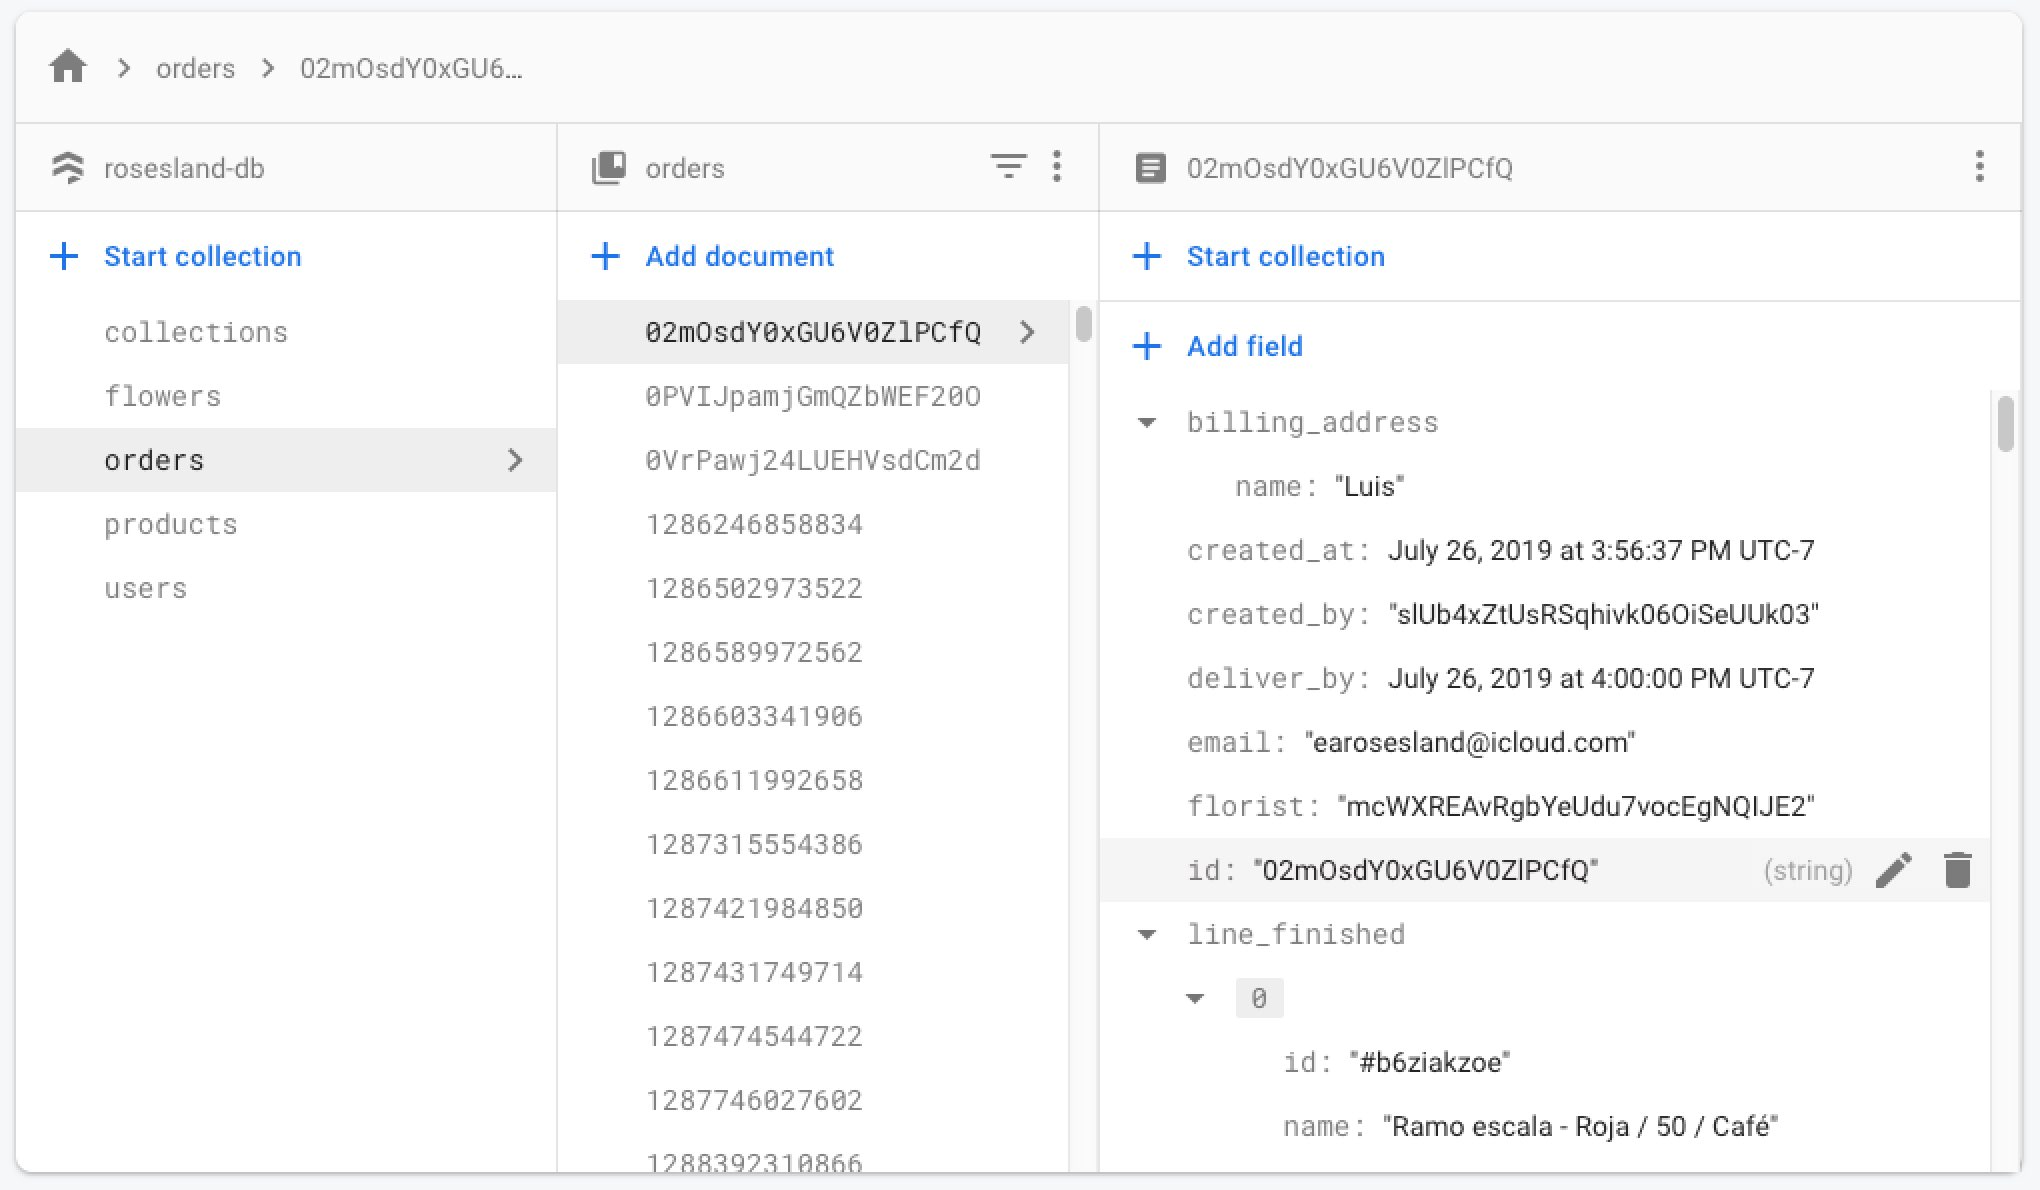
\includegraphics[width=0.9\textwidth]{firestore}
  \caption{Colección de Firestore con sus documentos internos.}
\end{figure}